

\documentclass[xcolor=x11names, compress,handout]{beamer}

%% General document %%%%%%%%%%%%%%%%%%%%%%%%%%%%%%%%%%
\usepackage{graphicx}
\graphicspath{{./img/}}


\usepackage{xcolor}

\usepackage{tikz}
\usetikzlibrary{positioning, arrows}
\usetikzlibrary{decorations.fractals}
\tikzstyle{every picture}+=[remember picture]
\tikzstyle{na} = [baseline=-.5ex]

\usepackage{pgfplots}
\pgfplotsset{compat=newest}
\usepgfplotslibrary{units}
\usepgfplotslibrary{external}
\usetikzlibrary{pgfplots.external}
% \tikzset{external/system call={latex \tikzexternalcheckshellescape 
% -interaction=batchmode -jobname "\image" "\texsource";
% dvips -o "\image".ps "\image".dvi;
% ps2eps "\image.ps"}}
% \tikzset{external/force remake}
\tikzexternalize[prefix=tikz/external/]



\usepackage{filemod}
\newcommand{\includetikz}[2]{%
  \tikzsetnextfilename{#2}%
  \filemodCmp{#1#2.tikz}{#1external/#2.pdf}%
    {\tikzset{external/remake next}}{}%
  \input{#1#2.tikz}%
}




\pgfplotsset{
  /pgfplots/scatter legend/.style={
    /pgfplots/legend image code/.code={\draw[##1,yshift=-0.1em] plot coordinates {
      (-0.1em, 0.1em)
      (0.2em, 0.45em)
      (0.3em, -0.05em)
      (0.6em, 0.3em)
    };},
    rounded corners=1.5pt,
  },
}


\usepackage{filecontents, anyfontsize, textcomp, siunitx}

\usepackage[super]{nth}


%%%%%%%%%%%%%%%%%%%%%%%%%%%%%%%%%%%%%%%%%%%%%%%%%%%%%%


%% Beamer Layout %%%%%%%%%%%%%%%%%%%%%%%%%%%%%%%%%%
%\useoutertheme[subsection=false,shadow]{miniframes}
\useoutertheme[subsection=false,shadow]{miniframes}
\usepackage{etoolbox}
\makeatletter
\patchcmd{\slideentry}
{\advance\beamer@xpos by1\relax}{}{}{}
\def\beamer@subsectionentry#1#2#3#4#5{\advance\beamer@xpos by1\relax}
\makeatother

%\setbeamertemplate{footline}{%
%\begin{beamercolorbox}{section in head/foot}
%    \color{gray}\vskip2pt~ \insertsection\hfill\insertpagenumber{} %
%    / \insertpresentationendpage{} ~\vskip2pt
%\end{beamercolorbox}
%}

\setbeamertemplate{footline}{%
\begin{beamercolorbox}{0}
    \color{black}\vskip2pt~ \hfill\insertframenumber{} \hspace{10pt} \vspace{3pt} ~\vskip2pt
\end{beamercolorbox}
}

\setbeamertemplate{navigation symbols}{}

\useinnertheme{default}
\usefonttheme{structuresmallcapsserif} % could be default, serif, structurebold, professionalfonts, structureitalicserif or structuresmallcapsserif
\usepackage{palatino}

\setbeamerfont{title like}{shape=\scshape}
\setbeamerfont{frametitle}{shape=\scshape}

\setbeamercolor*{lower separation line head}{bg=DeepSkyBlue4} 
\setbeamercolor*{normal text}{fg=black,bg=white} 
\setbeamercolor*{alerted text}{fg=red} 
\setbeamercolor*{example text}{fg=black} 
\setbeamercolor*{structure}{fg=black} 
 
\setbeamercolor*{palette tertiary}{fg=black,bg=black!10} 
\setbeamercolor*{palette quaternary}{fg=black,bg=black!10} 

\renewcommand{\(}{\begin{columns}}
\renewcommand{\)}{\end{columns}}
\newcommand{\<}[1]{\begin{column}{#1}}
\renewcommand{\>}{\end{column}}
%%%%%%%%%%%%%%%%%%%%%%%%%%%%%%%%%%%%%%%%%%%%%%%%%%


\AtBeginSection[]
{
  {
  \tikzexternaldisable
  \setbeamertemplate{footline}{}
  \begin{frame}[noframenumbering]{}
    \vfill
    \begin{center}
    \rmfamily \LARGE \insertsection
    \end{center}
        \begin{tikzpicture}[scale=0.1]
        % finalsectionnumber * delta = 115
        \pgfmathsetmacro\res{\insertsectionnumber * 28.75}
    \fill [lightgray] (9cm,0cm) rectangle (115cm,1cm);
    \fill [black] (9cm, 0cm) rectangle (\res cm,1cm);
    \end{tikzpicture}
    \vfill
  \end{frame}
  \tikzexternalenable
  }
}

\definecolor{lightgray}{gray}{0.75}
\definecolor{darkgreen}{RGB}{50,200,10}
\definecolor{aliceblue}{rgb}{0.94, 0.97, 1.0}
\newcommand{\ver}[1]{\texttt{\textbf{#1}}}
\everymath{\displaystyle}
\newcommand{\btVFill}{\vskip0pt plus 1filll}
\DeclareSIUnit\nat{nat}


\usepackage{listings}
% \lstset{
%   language=Python,
%   showstringspaces=false,
%   formfeed=newpage,
%   tabsize=4,
%   commentstyle=itshape,
%   morekeywords={models, lambda, forms}
% }

% \definecolor{keywords}{RGB}{255,0,90}
% \definecolor{comments}{RGB}{0,0,113}
% \definecolor{red}{RGB}{160,0,0}
% \definecolor{green}{RGB}{0,150,0}
% \lstset{language=Python, 
%         basicstyle=\ttfamily\small, 
%         keywordstyle=\color{keywords},
%         commentstyle=\color{comments},
%         stringstyle=\color{red},
%         showstringspaces=false,
%         identifierstyle=\color{green},
%         tabsize=4,
%         procnamekeys={def,class},
%         morekeywords={models, lambda, forms}
%       }

\usepackage{setspace}
\definecolor{Code}{rgb}{0,0,0}
\definecolor{Decorators}{rgb}{0.5,0.5,0.5}
\definecolor{Numbers}{rgb}{0.5,0,0}
\definecolor{MatchingBrackets}{rgb}{0.25,0.5,0.5}
\definecolor{Keywords}{rgb}{0,0,1}
\definecolor{self}{rgb}{0,0,0}
\definecolor{Strings}{rgb}{0,0.63,0}
\definecolor{Comments}{rgb}{0,0.63,1}
\definecolor{Backquotes}{rgb}{0,0,0}
\definecolor{Classname}{rgb}{0,0,0}
\definecolor{FunctionName}{rgb}{0,0,0}
\definecolor{Operators}{rgb}{0,0,0}
\definecolor{Background}{rgb}{0.98,0.98,0.98}
\lstnewenvironment{python}[1][]{
\lstset{
% numbers=left,
% numberstyle=\footnotesize,
% numbersep=1em,
xleftmargin=1em,
framextopmargin=2em,
framexbottommargin=2em,
showspaces=false,
showtabs=false,
showstringspaces=false,
% frame=l,
% tabsize=4,
tabsize=2,
% Basic
basicstyle=\ttfamily\small\setstretch{1},
backgroundcolor=\color{Background},
language=Python,
% Comments
commentstyle=\color{Comments}\slshape,
% Strings
stringstyle=\color{Strings},
morecomment=[s][\color{Strings}]{"""}{"""},
morecomment=[s][\color{Strings}]{'''}{'''},
% keywords
morekeywords={import,from,class,def,for,while,if,is,in,elif,else,not,and,or,print,break,continue,return,True,False,None,access,as,,del,except,exec,finally,global,import,lambda,pass,print,raise,try,assert},
keywordstyle={\color{Keywords}\bfseries},
% additional keywords
morekeywords={[2]@invariant},
keywordstyle={[2]\color{Decorators}\slshape},
emph={self},
emphstyle={\color{self}\slshape},
%
}}{}

\usepackage{minted}
\usemintedstyle{pastie}

\begin{document}


%%%%%%%%%%%%%%%%%%%%%%%%%%%%%%%%%%%%%%%%%%%%%%%%%%%%%%
%%%%%%%%%%%%%%%%%%%%%%%%%%%%%%%%%%%%%%%%%%%%%%%%%%%%%%
\begin{frame}[plain]
  \title{ {\fontsize{14}{1}\selectfont \bfseries Basic Python Tutorial} \\ \vspace{-3pt} {\fontsize{10}{1}\selectfont For Computational Neurodynamics Students} \\  }
\subtitle{ ~ }
\date{}
\vspace{5pt}
\titlepage
\vfill
\begin{center}

% {
% \tikzexternaldisable
%   \begin{tikzpicture}
%     \tikzstyle{inhib}=[-*, semithick, opacity=0.8, black!20!blue]
%     \tikzstyle{excit}=[-stealth', shorten >=1pt, opacity=0.8, semithick, black!20!blue]
%     \tikzstyle{synap}=[-stealth', gray!90!white, dashed]
%     \def\neuronR{1.6cm};
%     \def\netR{3cm}
% 
%       % \node[circle, fill=purple!50!black, opacity=0.2, minimum size=1.7*\neuronR] (INC) at (0:0cm) {};
%     \node[circle, thick, fill=blue!50!green] (titleInhib) at (0,0) {};
% 
%       \node[circle, fill=blue!60!green, opacity=0.4, minimum size=\neuronR] (titleExcit) at  (2,0) {};
%       \draw[inhib] (titleInhib) -- (titleExcit);
% 
%     \path[excit, bend left] (titleExcit) edge (titleInhib);
% 
%   \end{tikzpicture}
% 
% \tikzexternalenable
% }

  ~ \\
  
  \vfill
  {\large Pedro Mediano \hspace{30pt} Marta Garnelo}\\ \vspace{-8pt}
  {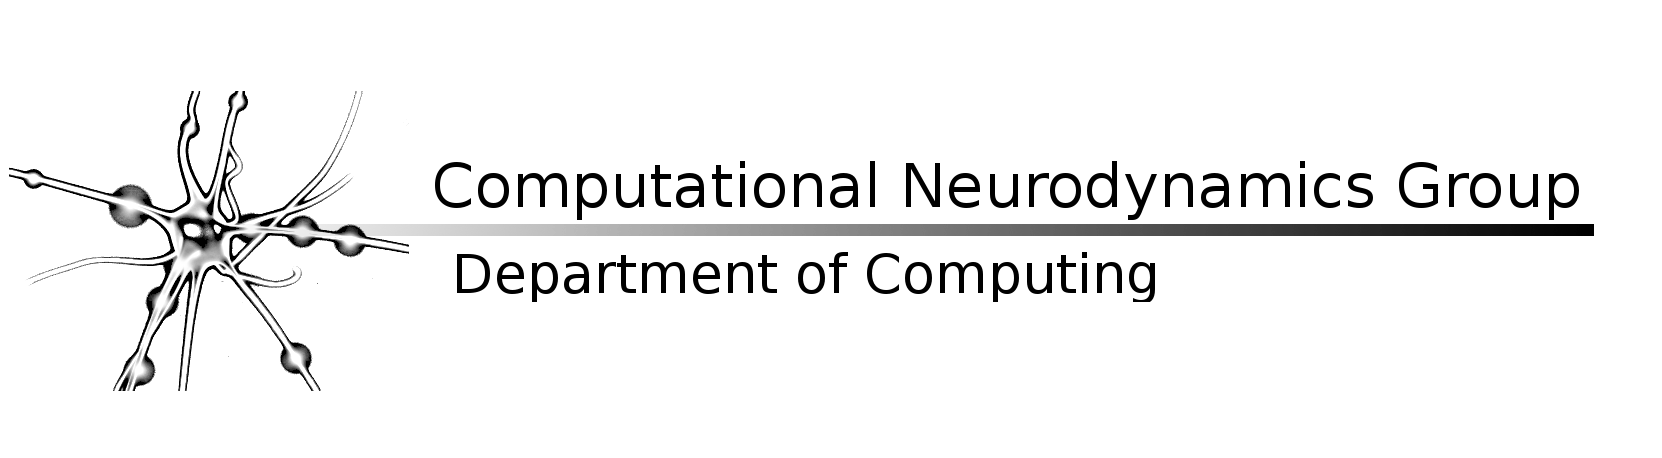
\includegraphics[width=0.7\textwidth]{logo3.png}}\\ \vspace{-10pt}


  \ver{pmediano@ic.ac.uk} \hspace{20pt} \ver{m.garnelo@ic.ac.uk}
\end{center}
\end{frame}


%%%%%%%%%%%%%%%%%%%%%%%%%%%%%%%%%%%%%%%%%%%%%%%%%%%%%%
%%%%%%%%%%%%%%%%%%%%%%%%%%%%%%%%%%%%%%%%%%%%%%%%%%%%%%
\section{ \scshape Introduction}
\subsection{Introduction}
\begin{frame}{}
\large

Completely legitimate question:

\vfill
\pause

\begin{itemize}
  \item \textbf{\Large Why are we using Python?}
\end{itemize}

\vfill

\end{frame}

%%%%%%%%%%%%%%%%%%%%%%%%%%%%%%%%%%%%%%%%%%%%%%%%%%%%%%
%%%%%%%%%%%%%%%%%%%%%%%%%%%%%%%%%%%%%%%%%%%%%%%%%%%%%%
\begin{frame}{Reasons to move to Python}

  (Or at least our reasons to do it)

  \begin{itemize}
    \Large
    \newcommand{\myitem}{\vfill \pause \item[{\color{darkgreen}\checkmark}]}
    \myitem It's free software.
    \myitem We know Python better than Matlab.
    \myitem We made the code better.
  \end{itemize}

\end{frame}


%%%%%%%%%%%%%%%%%%%%%%%%%%%%%%%%%%%%%%%%%%%%%%%%%%%%%%
%%%%%%%%%%%%%%%%%%%%%%%%%%%%%%%%%%%%%%%%%%%%%%%%%%%%%%
\section{\scshape Python basics}
\subsection{The import system}
\begin{frame}[fragile]{Python basics}

\textbf{The import system}

\begin{itemize}
	\item Often the definitions (e.g. functions) we want to use might be stored in a different script called \textit{module}.
	\item In order to use definitions from other modules we need to import these modules at the beginning of our script.
	\item This is done via the command \textit{import} 
% 			\begin{lstlisting}[xleftmargin=.2\textwidth]
% 				import numpy 
% 			\end{lstlisting}
  \mint{python}@    import numpy@
	\item If the name of the module is long we can set a new abbreviation for it
% 			\begin{lstlisting}[xleftmargin=.2\textwidth]
% 				import numpy as np
% 			\end{lstlisting}
  \mint{python}@    import numpy as np@
	\item We can also load specific definitions:
  \begin{minted}{python}
    from scipy import *
    from matplotlib import pyplot
  \end{minted}
\end{itemize}

\end{frame}


%%%%%%%%%%%%%%%%%%%%%%%%%%%%%%%%%%%%%%%%%%%%%%%%%%%%%%
%%%%%%%%%%%%%%%%%%%%%%%%%%%%%%%%%%%%%%%%%%%%%%%%%%%%%%
\subsection{\scshape Classes}
\begin{frame}[fragile]{Python basics}
\textbf{Classes}
\begin{itemize}
\item Classes are blueprints for creating objects
\item Classes can contain functions that are applied to objects from that class
\end{itemize}

\begin{minted}{python}
class Shape:
    def __init__(self, x , y):
        self.x = x
        self.y = y

    def area(self):
        return self.x * self.y

rectangle = Shape(100, 45)
print rectangle.area()
\end{minted}

\end{frame}

%%%%%%%%%%%%%%%%%%%%%%%%%%%%%%%%%%%%%%%%%%%%%%%%%%%%%%
%%%%%%%%%%%%%%%%%%%%%%%%%%%%%%%%%%%%%%%%%%%%%%%%%%%%%%
\subsection{Indentation}
\begin{frame}[fragile]{Python basics}
\textbf{Indentations in python}
\begin{itemize}
\item Indentations mark the blocks of code within script 
\item Each line of a block must be indented by the same amount
\end{itemize}

\begin{minted}{python}
if some_condition:
    if the_number == 4:
        do_something(fancy)
else:
    do_something(different)
\end{minted}

\begin{itemize}
\item Mind that beginnings of blocks are indicated with a colon ":"
\end{itemize}

\textbf{0 - indexing}
\begin{itemize}
\item The index of the first element in python is 0
\item Tip: "-1" refers to the last element 
\end{itemize}
\end{frame}


  
%%%%%%%%%%%%%%%%%%%%%%%%%%%%%%%%%%%%%%%%%%%%%%%%%%%%%%
%%%%%%%%%%%%%%%%%%%%%%%%%%%%%%%%%%%%%%%%%%%%%%%%%%%%%%
\section{ \scshape For Matlab Fans}
\begin{frame}{}
\large
\vspace{30pt}


First piece of advice:

% \vfill
\pause
\vspace{10pt}

\begin{itemize}
  \item \textbf{\Large Don't panic.}
\end{itemize}

\vspace{20pt}
% \btVFill

\begin{figure}[b]
  \centering
  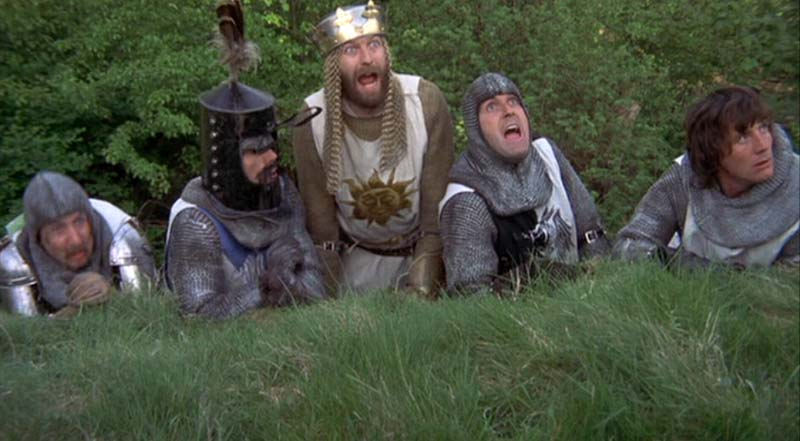
\includegraphics[width=\textwidth, clip, trim= 0 100 0 0]{HolyGrail072}
\end{figure}

\end{frame}

%%%%%%%%%%%%%%%%%%%%%%%%%%%%%%%%%%%%%%%%%%%%%%%%%%%%%%
%%%%%%%%%%%%%%%%%%%%%%%%%%%%%%%%%%%%%%%%%%%%%%%%%%%%%%
\begin{frame}[fragile]{General comments}
\textbf{Replacing Matlab with python}
\begin{itemize}
\item Overall Matlab and python are very similar in terms of syntax
\item \textbf{Similarities:} 
	\begin{enumerate}
	\item Both are \textit{dynamically typed} (every variable can contain data of any type)
	\item Both are \textit{interpreted}, they do not need to be compiled (almost)
	\end{enumerate}
\item \textbf{Differences}
	\begin{enumerate}
	\item Python files can contain unlimited functions that can all be accessed 
	\item Python does not have a matrix engine but there are useful packages with similar functionalities
		\begin{itemize}
		\item \textbf{Numpy}: enables basic matrix arithmetic on arrays
		\item \textbf{Scipy}: advanced mathematical routines
		\item \textbf{Matplotlib}: plotting
		\end{itemize}
	\end{enumerate}
\end{itemize}
\end{frame}


%%%%%%%%%%%%%%%%%%%%%%%%%%%%%%%%%%%%%%%%%%%%%%%%%%%%%%
%%%%%%%%%%%%%%%%%%%%%%%%%%%%%%%%%%%%%%%%%%%%%%%%%%%%%%
\subsection{Basic commands}
\begin{frame}{Basic commands}

  \large

  Most Matlab has direct correspondence in Python:

  \vspace{5pt}

  \begin{itemize}
    \newcommand{\myitem}{\vspace{3pt} \pause \item}
    \myitem Variable declaration
    \myitem Loops
    \myitem Flow control
    \myitem Function handles
    \myitem That's it!
  \end{itemize}

\end{frame}

%%%%%%%%%%%%%%%%%%%%%%%%%%%%%%%%%%%%%%%%%%%%%%%%%%%%%%
%%%%%%%%%%%%%%%%%%%%%%%%%%%%%%%%%%%%%%%%%%%%%%%%%%%%%%
\subsection{Data structures}
\begin{frame}[fragile]{Common data structures}

  \large
  \vspace{-5pt}

  \begin{description}
    \item[Python] ~ \\ \hspace{-30pt} Lists, dictionaries, arrays, \ldots
    \vspace{8pt}
    \item[Matlab] ~ \\ \hspace{-30pt} Arrays, cells, structs, \ldots
  \end{description}

  \vspace{10pt}

  \(
  \<{0.6\linewidth}

  \centering
  \textbf{Python}
  \begin{minted}{python}
    A = [1,3,2,4]
    B = {'a': 0.2,
         'b': 0.02}
    C = np.array([10,20])
  \end{minted}

  \> \<{0.6\linewidth}

  \centering
  \textbf{Matlab}
  \begin{minted}[frame=leftline]{octave}
    A = [1,3,2,4];
    B.a = 0.1;
    B.b = 0.02;
    C = [10,20];
  \end{minted}

  \>
  \)

  \vspace{25pt}

  We recommend to use always \textbf{\texttt{np.array}}.

\end{frame}

%%%%%%%%%%%%%%%%%%%%%%%%%%%%%%%%%%%%%%%%%%%%%%%%%%%%%%
%%%%%%%%%%%%%%%%%%%%%%%%%%%%%%%%%%%%%%%%%%%%%%%%%%%%%%
\subsection{The Question}
\begin{frame}{The big question}

  \large

  \textbf{\Large Can I use Matlab?}

  \vspace{20pt}
  \pause

  Yes, but:

  \vspace{3pt}

  \begin{itemize}
    \newcommand{\myitem}{\vspace{3pt} \pause \item[{\color{darkgreen}\checkmark}]}
    \newcommand{\baditem}{\vspace{3pt} \pause \item[{\color{red}$\boldsymbol\times$}]}
    \baditem The Matlab code is not maintained.
    \baditem Matlab makes the markers sad.
    \baditem We provide limited support for Matlab questions.
    \myitem Come on, use Python.
  \end{itemize}

\end{frame}


%%%%%%%%%%%%%%%%%%%%%%%%%%%%%%%%%%%%%%%%%%%%%%%%%%%%%%
%%%%%%%%%%%%%%%%%%%%%%%%%%%%%%%%%%%%%%%%%%%%%%%%%%%%%%
\section{ \scshape Tools}
\subsection{Development environments}
\begin{frame}{Development environments}

  \large
  \begin{itemize}
    \item Vim + terminal
    \item Spyder
    \item Atom
  \end{itemize}

  Remember to use a debugger! \\
  ~ ~ $\rightarrow$ \textbf{pdb}

\end{frame}

%%%%%%%%%%%%%%%%%%%%%%%%%%%%%%%%%%%%%%%%%%%%%%%%%%%%%%
%%%%%%%%%%%%%%%%%%%%%%%%%%%%%%%%%%%%%%%%%%%%%%%%%%%%%%
\subsection{Virtual environments and packages}
\begin{frame}{Logistics}

  \large

  \vfill

  \begin{itemize}
     
    \item If you still don't have access to the DoC machines, talk with me ASAP!

  \vfill

    \item No mortal is allowed to install programs on the DoC machines, so we'll
  use Python's \textbf{virtualenv}.

  \begin{itemize}
    \item A \emph{virtual environment} is a Python island.
    \item You can~ \ver{pip install} packages inside without requiring permissions.
  \end{itemize}

  \end{itemize}

  \vfill
  ~
  \vfill

\end{frame}

%%%%%%%%%%%%%%%%%%%%%%%%%%%%%%%%%%%%%%%%%%%%%%%%%%%%%%
%%%%%%%%%%%%%%%%%%%%%%%%%%%%%%%%%%%%%%%%%%%%%%%%%%%%%%
\begin{frame}[fragile]{Virtual environments and new packages}

  \begin{itemize}
    \item Setting up your \ver{virtualenv}:
  \end{itemize}
  \begin{minted}[bgcolor=aliceblue]{bash}
    cd /vol/bitbucket
    mkdir <YOURUSERNAME>
    cd <YOURUSERNAME>
    virtualenv venv
    cd venv
    source bin/activate
    pip install scipy
    pip install matplotlib
    pip install jpype1
  \end{minted}

\end{frame}

%%%%%%%%%%%%%%%%%%%%%%%%%%%%%%%%%%%%%%%%%%%%%%%%%%%%%%
%%%%%%%%%%%%%%%%%%%%%%%%%%%%%%%%%%%%%%%%%%%%%%%%%%%%%%
\begin{frame}[fragile]{Virtual environments and new packages}

  \begin{itemize}
    \item To install Spyder:
  \end{itemize}
  \begin{minted}[bgcolor=aliceblue]{bash}
    pip install PySide
    pip install spyder
  \end{minted}

  \vspace{10pt}

  \begin{itemize}
    \item Using the \ver{virtualenv}:
  \end{itemize}
  \begin{minted}[bgcolor=aliceblue]{bash}
    source /<PATHTOVENV>/bin/activate
    python EulerDemo.py
    spyder
  \end{minted}
  
\end{frame}

%%%%%%%%%%%%%%%%%%%%%%%%%%%%%%%%%%%%%%%%%%%%%%%%%%%%%%
%%%%%%%%%%%%%%%%%%%%%%%%%%%%%%%%%%%%%%%%%%%%%%%%%%%%%%
\subsection{Links}
\begin{frame}{Useful links}

  \large

  \begin{itemize}
    \item NumPy for Matlab users:

    \vspace{5pt}
    {\scriptsize \centering \url{http://wiki.scipy.org/NumPy_for_Matlab_Users}\\}

    \vspace{8pt}
    \item Using Vim as a Python IDE:

    \vspace{5pt}
    {\scriptsize \centering \url{https://www.youtube.com/watch?v=YhqsjUUHj6g} \\
    \url{http://blog.dispatched.ch/2009/05/24/vim-as-python-ide/}}

    \vspace{8pt}
    \item The Python tutorial:

    \vspace{5pt}
    {\scriptsize \centering \url{https://docs.python.org/2/tutorial/}\\}

  \end{itemize}


\end{frame}

%%%%%%%%%%%%%%%%%%%%%%%%%%%%%%%%%%%%%%%%%%%%%%%%%%%%%%
%%%%%%%%%%%%%%%%%%%%%%%%%%%%%%%%%%%%%%%%%%%%%%%%%%%%%%
\section{}
\begin{frame}{Live example}

  \Large

  Let's go through \ver{IzNeuronDemo.py}

\end{frame}

%%%%%%%%%%%%%%%%%%%%%%%%%%%%%%%%%%%%%%%%%%%%%%%%%%%%%%
%%%%%%%%%%%%%%%%%%%%%%%%%%%%%%%%%%%%%%%%%%%%%%%%%%%%%%
{
  \setbeamercolor{background canvas}{bg=black}
  \usebackgroundtemplate{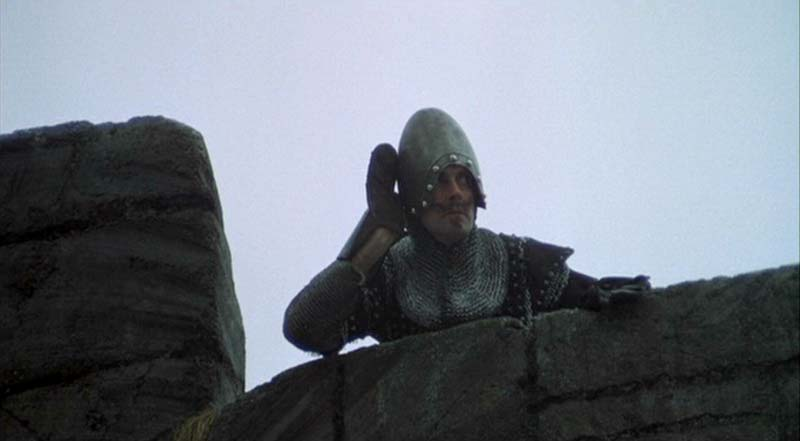
\includegraphics[width=\paperwidth, clip, trim=80 0 80 0]{HolyGrail065}}
\begin{frame}[plain, noframenumbering]
\end{frame}
}


\end{document}

